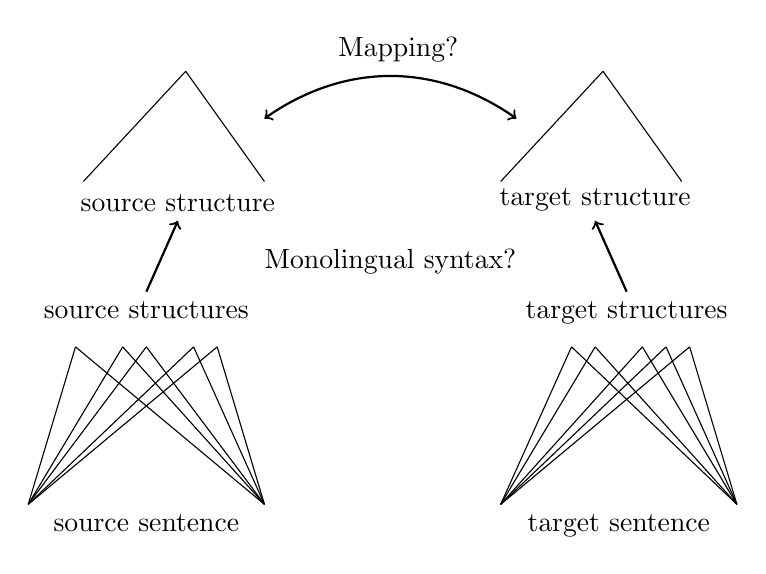
\begin{tikzpicture}

\coordinate (ss) at (1.5,0);
\node [below] at (ss) {source sentence};
\coordinate (ts) at (7.5,0);
\node [below] at (ts) {target sentence};

%source trees
\draw (0,0) -- (0.6,2) (3,0) -- (0.6,2);
\draw (0,0) -- (1.2,2) (3,0) -- (1.2,2);
\draw (0,0) -- (1.5,2) (3,0) -- (1.5,2);
\draw (0,0) -- (2.1,2) (3,0) -- (2.1,2);
\draw (0,0) -- (2.4,2) (3,0) -- (2.4,2);

%target trees
\draw (6,0) -- (6.9,2) (9,0) -- (6.9,2);
\draw (6,0) -- (7.2,2) (9,0) -- (7.2,2);
\draw (6,0) -- (7.8,2) (9,0) -- (7.8,2);
\draw (6,0) -- (8.1,2) (9,0) -- (8.1,2);
\draw (6,0) -- (8.4,2) (9,0) -- (8.4,2);


\coordinate (sstruct) at (1.5,2.7);
\coordinate (tstruct) at ((7.6,2.7);
\coordinate (syntax) at ((4.6,2.8);
\coordinate (1sstruct) at (1.9,3.6);
\coordinate (1tstruct) at (7.2,3.6);

\node [below] at (sstruct) {source structures};
\node [below] at (tstruct) {target structures};
\node [above] at (1sstruct) {source structure};
\node [above] at (1tstruct) {target structure};
\node [above] at (syntax) {Monolingual syntax?};
\node [above] at (4.7,5.5) {Mapping?};

%draw source tree
\draw (0.7,4.1) --(2.0,5.5) (3.0,4.1) --(2.0,5.5);
\draw (6.0,4.1) --(7.3,5.5) (8.3,4.1) --(7.3,5.5);

\draw[->,thick] (sstruct) to (1sstruct);
\draw[->,thick] (tstruct) to (1tstruct);
\draw[<->, bend left = 35, thick] (3.0,4.9) to (6.2,4.9);

\end{tikzpicture}